\documentclass[letterpaper]{article}

\usepackage{hyperref,natbib,alifeconf,listings,subcaption,textcomp,xcolor}  %% The order is important - natbib must be before alifeconf

% Automatic formatting of SI units
\usepackage[binary-units]{siunitx}

% Configure listing
\lstset{language=C++,showstringspaces=false,upquote=true,identifierstyle=\ttfamily\color{black}}

% Visible TODO notes
\newcommand{\todo}[1]{\textbf{\textsc{\textcolor{red}{(TODO: #1)}}}}

% *****************
%  Requirements:
% *****************
%
% - All pages sized consistently at 8.5 x 11 inches (US letter size).
% - PDF length <= 8 pages for full papers, <=2 pages for extended
%    abstracts.
% - Abstract length <= 250 words.
% - No visible crop marks.
% - Images at no greater than 300 dpi, scaled at 100%.
% - Embedded open type fonts only.
% - All layers flattened.
% - No attachments.
% - All desired links active in the files.

% Note that the PDF file must not exceed 5 MB if it is to be indexed
% by Google Scholar. Additional information about Google Scholar
% can be found here:
% http://www.google.com/intl/en/scholar/inclusion.html.


% If your system does not generate letter format documents by default,
% you can use the following workflow:
% latex example
% bibtex example
% latex example ; latex example
% dvips -o example.ps -t letterSize example.dvi
% ps2pdf example.ps example.pdf


% For pdflatex users:
% The alifeconf style file loads the "graphicx" package, and
% this may lead some users of pdflatex to experience problems.
% These can be fixed by editing the alifeconf.sty file to specify:
% \usepackage[pdftex]{graphicx}
%   instead of
% \usepackage{graphicx}.
% The PDF output generated by pdflatex should match the required
% specifications and obviously the dvips and ps2pdf steps become
% unnecessary.


% Note:  Some laser printers have a serious problem printing TeX
% output. The use of ps type I fonts should avoid this problem.


\title{Critical Exponent of Species-Size Distribution in Evolution}
\author{James C. Knight$^{1}$ \and Andrew Philippides$^{1}$ \\
\mbox{}\\
$^1$Centre for Computational Neuroscience and Robotics, University of Sussex, Brighton, UK \\
J.C.Knight@sussex.ac.uk} % email of corresponding author

% For several authors from the same institution use the same number to
% refer to one address.
%
% If the names do not fit well on one line use
%         Author 1, Author 2 ... \\ {\Large\bf Author n} ...\\ ...
%
% If the title and author information do not fit in the area
% allocated, place \setlength\titlebox{<new height>} after the
% \documentclass line where <new height> is 2.25in



\begin{document}
\maketitle

\begin{abstract}
% Abstract length should not exceed 250 words
Inspired by the visual scanning behaviour seen in ants, models of visually-guided navigation that operate by searching for previously experienced views of the world, have been shown to be capable of facilitating robust navigation.
However, these algorithms have only been previously tested using simulated agents in virtual environments, not on natural scenes or physical robotic agents.\todo{Andy is this true? living machines paper does look at natural scenes but not really navigation. }
In this work we explore the performance of these algorithms both offline, using a dataset consisting of images and video routes captured in an outdoor environment, and running onboard an autonomous robot.
The results from our experiments show that these insect-inspired algorithms are capable of extracting reliable direction information even when scenes contain few local landmarks and high-levels of noise.
Furthermore, when running these algorithms on our autonomous robot, we demonstrate that routes can be successfully recapitulated precisely -- our robot remains an average of only \SI{10}{\centi\metre} away from the trained path.
\end{abstract}

\section{Introduction}
dd

\section{Methods}
\subsection{Familiarity-driven navigation algorithms}
\label{sec:navigation_algorithms}
\begin{itemize}
    \item PerfectMemory
    \item InfoMax
\end{itemize}

\begin{figure}[t]
    \centering
    \includegraphics[width=2in]{figures/robot.jpg}
    \caption{Robot platform with onboard computation.}
    \label{fig:robot}
\end{figure}

\subsection{Robot platform}
\label{sec:robot_platform}
In this work we use the robot platform developed by \citet{Domcsek2018} shown in figure~\ref{fig:robot}.
This robot is based on a Parallax `Shield-Bot' chassis~\citep{ParallaxInc}, with a Jetson TX1 embedded computer~\citep{NVIDIACorporation2016} mounted on top for additional onboard computation and additional batteries mounted underneath. 
The Jetson TX1 is connected via USB to a Kodak PixPro SP360 4K camera~\citep{JKImagingLtd}, mounted on top of the robot connected which provides panoramic visual input.

\begin{figure}[t]
    \begin{subfigure}[b]{\columnwidth}
        \includegraphics[width=\columnwidth]{figures/360_240.jpg}
        \caption{Unprocessed panoramic image}
    \end{subfigure}
    \begin{subfigure}[b]{\columnwidth}
        \includegraphics[width=\columnwidth]{figures/360_240_mask.png}
        \caption{Sky-segmented panoramic image}
    \end{subfigure}
    \caption{Example panoramic images from our database}
    \label{fig:database_images}
\end{figure}

\subsection{Image database}
\label{sec:image_database}
Using a Kodak PixPro SP360 4K panoramic camera~\citep{JKImagingLtd}, we recorded 195 images of the ‘Library Square’ at the University of Sussex (figure?). 
These were taken on a \SI{1.2}{\metre} grid, defined by square’s paving slabs. 
Alongside this reference grid, we also recorded videos from the same camera, mounted on the mobile robot described in the previous section, while we manually drove it along six routes of varying tortuosity across the square. 
As well as these videos, taken from the robot’s point-of-view, we simultaneously recorded the position of the robot using a camera mounted on a tripod. 
After synchronising these videos, we extracted the position of the robot over time using the Discriminative Correlation Filter Tracker with Channel and Spatial Reliability~\citep{Lukezic2018} implementation provided by OpenCV~\citep{OpenCV}.
Finally, we again used OpenCV to apply a perspective transform to the positions extracted by the tracker and synchronised these final positions with the video frames captured by the robot. 
\citet{Stone2014} showed that sky-segmented, binary images can be used for robust visual navigation and, while our robot does not have a suitable UV camera, by using the watershed segmentation algorithm~\citep{Beucher1979} with markers placed at the top and bottom of each image, we obtained automatically sky-segmented versions of all of the images in our dataset.
Figure~\ref{fig:database_images} shows some example images from this database.

\begin{figure*}[t]
    \centering
    \begin{subfigure}[t]{0.3\textwidth}
        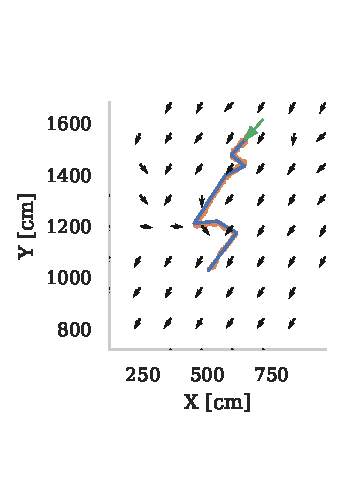
\includegraphics{figures/vector_field_route2_PerfectMemory_mask.eps}
        \caption{Simple route}
        \label{fig:vector_fields/route2_perfect_memory_mask}
    \end{subfigure}
    \begin{subfigure}[t]{0.3\textwidth}
        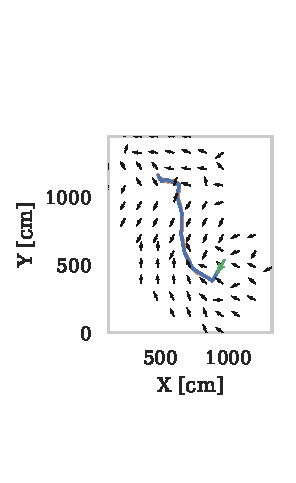
\includegraphics{figures/vector_field_route5_PerfectMemory_mask.eps}
        \caption{Longer route where visual aliasing occurs in the middle section}
        \label{fig:vector_fields/route5_perfect_memory_mask}
    \end{subfigure}
    \begin{subfigure}[t]{0.3\textwidth}
        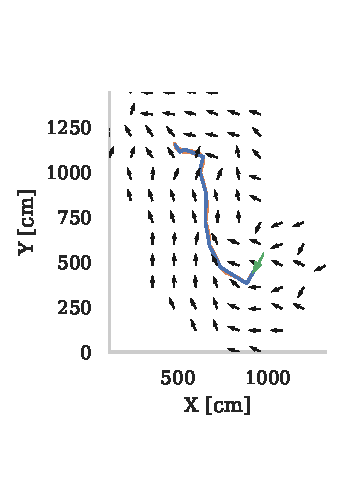
\includegraphics{figures/vector_field_route5_PerfectMemoryConstrained_mask.eps}
        \caption{By only considering rotated views within 90° of the route, visual aliasing can be avoided}
        \label{fig:vector_fields/route5_perfect_memory_constrained_mask}
    \end{subfigure}
    
    \caption{Vector fields showing the directions an agent, trained on a route, would move at each point within 4m of the route using a Perfect Memory algorithm with the skyline extracted using the watershed algorithm. 
    Orange lines shows data from our camera-based tracking of the robot and blue shows the version simplified using the Ramer-Douglas-Peucker algorithm~\citep{Ramer1972}}
    \label{fig:vector_fields}
\end{figure*}

\begin{figure}[t]
    \begin{subfigure}[b]{\columnwidth}
        \includegraphics[width=\columnwidth]{figures/alias_ridf.eps}
        \caption{Rotational Image Difference function}
        \label{fig:aliasing/ridf}
    \end{subfigure}
    
    \begin{subfigure}[b]{\columnwidth}
        \includegraphics[width=\columnwidth]{figures/image_diff_bad.png}
        \caption{Difference image with visual aliased route image}
        \label{fig:aliasing/image_diff_bad}
    \end{subfigure}
    
    \begin{subfigure}[b]{\columnwidth}
        \includegraphics[width=\columnwidth]{figures/image_diff_good.png}
        \caption{Difference image with correct route image}
        \label{fig:aliasing/image_diff_good}
    \end{subfigure}
    \caption{Analysis of aliasing shown in figure~\ref{fig:vector_fields/route5_perfect_memory_mask}.
    Using grid image taken at (\SI{600}{\metre}, \SI{720}{\metre}).
    All images were preprocessed using watershed segmentation algorithm.}
    \label{fig:aliasing}
\end{figure}

\section{Results}
\subsection{Image database}
We trained both the InfoMax and Perfect Memory algorithms on the images taken along the six routes in our dataset and then used them to find the direction a robot would move when placed at each grid point within \SI{4}{\metre} of the trained route. 
Heading direction were calculated by rotating the grid image taken at a point through \SI{\pm 180}{\degree} and finding the angle at which the algorithm reported the highest familiarity.
Figure~\ref{fig:vector_fields} shows some example vector fields obtained by plotting this direction at each of the chosen grid locations when using the Perfect Memory algorithm with the watershed segmentation-based preprocessing discussed in section~\ref{sec:image_database}. 
While the vector field suggests that the route shown in Figure~\ref{fig:vector_fields/route2_perfect_memory_mask} would be recapitulated successfully, in the middle section of the route shown in Figure~\ref{fig:vector_fields/route5_perfect_memory_mask}, errors occur.
Figure~\ref{fig:aliasing/ridf} shows a Rotational Image Difference Function~(RIDF) taken at one of the problematic locations on this route \todo{mark grid and add arrows showing aliases} (\SI{600}{\metre}, \SI{720}{\metre}) and it is clear that, as well as the local minima representing the correct heading at \SI{15}{\degree}, there is an additional, slightly lower local minima at \SI{153}{\degree} which is overriding the correct choice.
Figures~\ref{fig:aliasing/image_diff_bad}~and~\ref{fig:aliasing/image_diff_good} show the per-pixel differences between the two route images and the rotated versions of the grid image which correspond with these minima and this makes the cause of the problem become clear.
Although the \emph{shapes} of the skylines in figure~\ref{fig:aliasing/image_diff_good} are clearly more similar than those in figure~\ref{fig:aliasing/image_diff_bad}, there is a vertical offset -- probably caused by camera shake -- which introduces a large difference between the two images.

\begin{figure*}[t]
    \centering
    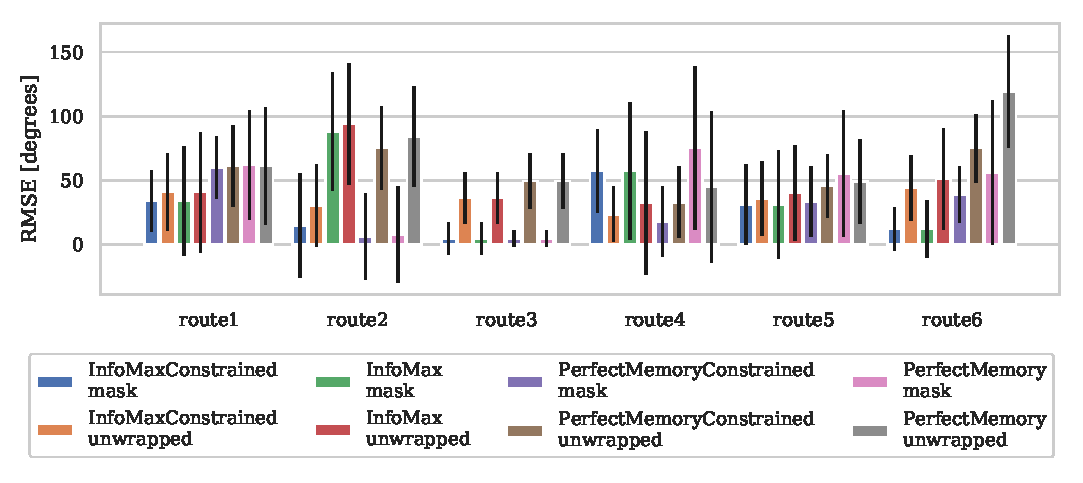
\includegraphics{figures/route_benchmark.eps}
    \caption{Performance of different algorithms on each of the 6 routes. \todo{decide on consistent names for routes}}
    \label{fig:route_benchmark}
\end{figure*}

However, if we were recapitulating the route using a real robot, these false-positive matches could be eliminated and computation saved by not scanning the full \SI{\pm 180}{\degree}. 
We can simulate this using our existing database of images by first making a simplified version of each route using the Ramer-Douglas-Peucker algorithm~\citep{Ramer1972} and determining the direction of each of the resultant segments.
Using these headings, we can then ignore matches that would involve heading more than \SI{\pm 90}{\degree} away from the direction of the nearest section of the route.
Figure~\ref{fig:vector_fields/route5_perfect_memory_constrained_mask} shows that this step solves the aliasing problems in this particular case and figure~\ref{fig:route_benchmark} confirms that this is the case across all algorithms and routes.
Furthermore, figure~\ref{fig:route_benchmark} also shows that, when using the Perfect Memory algorithm, sky-segmentation improves performance for almost all routes.
This improvement is less significant when using the InfoMax algorithm but, 

\begin{figure}[t]
    \centering
    \includegraphics{figures/jetson_test_performance.eps}
    \caption{Performance of visual navigation algorithms running on Jetson TX1. 
    Reported times are measured using \lstinline{std::chrono::high_resolution_clock} and average is taken over \num{100} images.}
    \label{fig:jetson_test_performance}
\end{figure}

\subsection{Performance of algorithm}
In the previous section, we showed that these simple insect-inspired algorithms are capable of robustly extracting heading direction in outdoor scenes. 
However, in order to deploy these algorithms on a real robot with constrained on board processing, their performance is important. 


\begin{figure}[t]
    \centering
    \includegraphics[width=2in]{figures/robot_environment.jpg}
    \caption{Environment used for robot testing.}
    \label{fig:robot_environment}
\end{figure}

\begin{figure}[t]
    \centering
    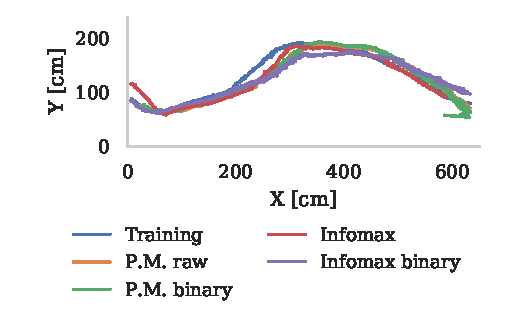
\includegraphics{figures/robot_paths.eps}
    \caption{Reconstructed paths of autonomous robot during training and testing using each algorithm.}
    \label{fig:robot_paths}
\end{figure}


\subsection{Autonomous robot}
Using the implementations of InfoMax and the Perfect Memory algorithms from our Brains-on-Board Robotics **ref** library, we built a simple application which can recapitulate learned routes on the robot described in section~\ref{sec:robot_platform} by running the following simple algorithm every \SI{500}{\milli\second} (based on the performance for 1000 images established in the previous section):
\begin{enumerate}
    \item Capture and unwrap a panoramic image.
    \item Perform one of the image processing steps described in section~\ref{sec:image_database}.
    \item Using either the InfoMax or Perfect Memory algorithm, calculate the familiarity with the processed image ‘in-silico’ when rotated through \SI{\pm 90}{\degree}°.
    \item Find the orientation with the highest familiarity and, if it is within \SI{4}{\degree} \todo{CHECK}, start driving forwards, otherwise start turning in the correct direction to align with the image.
\end{enumerate}
In order to compare the performance of the navigation algorithms and image processing steps described in sections~\ref{sec:navigation_algorithms}~and~\ref{sec:image_database} when using this algorithm, we first manually drove the robot along a sinuous route through the wooded area shown in figure~\ref{fig:robot_environment}, recording training images every \SI{100}{\milli\second}\todo{check} (resulting in a dataset of \num{455} images).
We then trained each of the navigation algorithms on this dataset and allowed the robot to recapitulate the path using the procedure described above.
Throughout this training and testing process, we used the same method described in section~\ref{sec:image_database} to track the robot resulting in the data shown in figure~\ref{fig:robot_paths}.
The robot was able to successfully recapitulate the training path using each of the navigation and image processing algorithms with little difference in performance immediately apparent in figure~\ref{fig:robot_paths}.
We confirmed this by calculating the shortest distance to the training path at each location along each recapitulated path and found that, in this environment, there was no significant difference between the performance of the different algorithms and overall the mean of the distance between the training and recapitulated paths was \SI{9}{\centi\metre}, with a standard deviation of \SI{8}{\centi\metre}.

\section{Discussion}
\begin{itemize}
    \item how/why SLAM is the obvious alternative
    \item General limitations of monocular SLAM
\end{itemize}
Typically, visual SLAM implementations extract features such as SURF or SIFT which require several hundreds of milliseconds to extract per frame~\citep{Bay2006}. 
This makes such implementations impractical to use in real-time, especially on constrained mobile platforms. 
However, more recent SLAM implementations such as FLaME~\citep{Greene2017} have been shown to run on autonomous quadrotors in only around \SI{10}{\milli\second} per frame. 
While this is significantly faster than our current InfoMax implementation, \citet{Greene2017} were using a much more powerful Intel CPU on their quadrotor (\citet{Biddulph2018} measure these devices as being $5\times$ faster than a Jetson TX1). 
For consistency we used $120 \times 25$ pixel images for all of the work presented in this paper but, when \citet{Baddeley2012} first demonstrated InfoMax for visual navigation, they used input images with around half this number of pixels.
Because the time taken to calculate the matrix-vector product required for equation~\todo{reference} scales quadratically, using input images with half the number of pixels would quarter the time taken to evaluate equation~\todo{reference}.
Furthermore, while our InfoMax implementation uses OpenMP~\todo{citation} to take advantage of the the Jetson TX1's four CPU cores, it does not utilise the \num{256} core GPU present on the Jetson TX1.
Initial experiments using the cuBLAS~\citep{NVIDIACorporation2007} GPU-accelerated linear algebra library suggest that InfoMax inference could be performed in around \SI{100}{\milli\second} for $120 \times 25$ pixel images.

\section{Conclusions}
ss
\section{Acknowledgements}
This work was funded by the EPSRC (Brains on Board project, grant number EP/P006094/1).
We would also like to thank Daniil Sakhapov for his work collecting the `library square' database of images, Alex Dewar for developing the BoB robotics framework and Norbert Domcsek for assisting with the data collection for this paper. 

\footnotesize
\bibliographystyle{apalike}
\bibliography{alife} % replace by the name of your .bib file


\end{document}
